% !TEX root = ../thesis.tex
%
\chapter{Evaluation}
\label{ch:evaluation}

%Research question for \acf{IFAS}, WIP: "\todo{not specific enough}Can \ac{IFAS} be used to capture and analyze passive user feedback?"

Checks wether the goals in \cref{sec:design:goals} are fulfilled.

[Blurb about user tests ...]

Additionally, a performance test shall ensure that \acf{IFAS} is able to handle large amounts of user feedback, both during processing as well as when visualizing the results in Kibana.
For this purpose, 10.000\todo{number not final} \texttt{UserClicked} events with random click coordinates are created and sent to Event Store by an application explicitly built for this objective.
Details about this test can be found in \cref{sec:evaluation:performance}.

% aus \cite{Easterbrook2008a} - What kind of research question are you asking?

\section{User Test}
\label{sec:evaluation:user}

In order to test the validity of \ac{IFAS} for collecting and analyzing implicit user feedback, a usability test was executed.
This testing method was chosen because usability tests allow for very specific guidance of the user through the application.
However, it should be explicitly noted that this test does not have the goal of evaluating the usability of the modified Mattermost client.
Instead, the results should show that \ac{IFAS} works as intended for implicit feedback in general and for controlled experiments in particular.

The experiment serves to prove three features of \ac{IFAS}.
First, the system can be used to monitor application usage in general.
This is shown by visualizing click events and data about sent chat messages.
Second, the system can be used to monitor the users' acceptance of specific application features.
This is shown by capturing usage data of two different mechanics for achieving the same result (switching chat channels).
Third, the system allows experimenters to perform controlled experiments, especially A/B tests.
This is shown by performing an A/B test within the usability test.
It should be noted that while the sample size for this experiment is sufficient for a usability test, it is way too low if a real world A/B test where to be executed because the collected data would be statistically irrelevant.
This is not a problem because the experiment is merely used to prove that \ac{IFAS} allows for collection and analysis of A/B test data; the performance test (cf. \cref{sec:evaluation:performance}) proves that the system is also able to handle enough events for an A/B test to be statistically relevant.
An A/A test is also done in order to prove the validity of the randomization unit.

Sample size of 10 user -- more than enough~\cite{Turner2006}.

- give user a test document with login information for Mattermost

- test document contains explicit tasks such as "send a DM to user Janis"

- task 0: If you have not used Mattermost before, please go through the brief tutorial (number of users who do the tutorial is monitored)

- task 1: Switch to the channel X. Then: Switch to Channel Y using the channel switcher (via Ctrl+K / CMD+K or the "channel switcher" button at the bottom left). Then: Switch to channel Z - user now knows both approaches for switching channels, which is used more often? Is the "channel switcher" feature used at all during regular usage?

- task 2: Another controlled experiment, similar to task 1.

- Task 3: A more open-ended tasks such as "browse a channel that is of interest to you for one minute"(?).
Each channel has some channel history (need some content for this, maybe some images or short stories (in chat form) under public domain).
This allows for predictions which content is more interesting for the users.
This leads to scrolling if the test subject finds the contents interesting, which has been shown to correlate strongly with interest in the page \cite{Claypool2001}.

- This also leads to general usage of the chat application, which allows for general passive user feedback via \texttt{UserClicked} events etc.
Need more data, what to collect? (e.g. amount of messages, types of messages)

% Thoughts regarding \cite{dumas2009usability}
% is this a diagnostic test, i.e. no statistically relevant outcome can be concluded from them?
% OR is this more like a validation test for establishing wether the system meets some usability requirements
% OR is usability testing just not the right fit for this? I kind of just need to simulate real user behavior, but not in a statistically relevant way, more like for a POC
%
% this is an asynchronous remote test

\subsection{Experimental Set-Up}

For the experiment, the web version of the Mattermost client was modified in order to send the desired events to \ac{IFAS}.
This involves both implicit feedback events in general as well as very specific events for controlled experiments.
I detail, the experiment involves the following aspects\todo{?}:

\begin{description}
\item[Click analysis (monitoring)] Every click that the user does during the usability test is sent to \ac{IFAS} as a \texttt{UserClickedEvent}.
This data is visualized in two ways in Kibana.
First, a click heatmap (cf. \cref{fig:evaluation:user:click-heatmap}) visualizes where the users interact with the application.
Second, in a line chart which displays a users click rate over time
\item[Channel usage (monitoring)]
\item[Usage of the channel switcher (feature analysis)]
\item[Click rate of a modified tutorial button (A/B test)]
\item[Click rate of the login button (A/A test]
\end{description}


 % explain how this does not suffice as a real controlled experiment (for example, sample size is not large enough) but still suffices to *simulate* a controlled experiment and prove that the necessary results are measured in IFAS -- use some Kohavi ref.

\subsection{Execution}

\subsection{Results}

\paragraph{Click Analysis}

...

It should be noted that the created click heatmap assumes a resolution of 1920x1080 pixels, which very certainly differs from the actual window size that the test subjects use.
Thus, if such a visualization where to be used in a production environment, the click coordinates would have to be normalized by a factor dependent on the user's window size.
This should be possible with relative ease using Elasticsearch's bucket aggregations, but was not implemented for this thesis due to its additional complexity and resulting time constraints.

%\begin{figure}[htb]
%        \includegraphics[width=\textwidth]{gfx/click-heatmap}
%        \caption{Click Heatmap}
%        \label{fig:evaluation:user:click-heatmap}
%\end{figure}


\section{Performance Test}
\label{sec:evaluation:performance}

TODO: Do the performance test for an A/B test!

For the purpose of testing the performance of \ac{IFAS}, a predefined number of \texttt{UserClicked} events was created and sent to the Event Store instance in rapid succession.
This causes a dedicated persistent subscription, which the Event Store-Elasticsearch bridge listens on, to forward the events, which in turn causes the events being fed into Elasticsearch as fast as possible.
A visualization of the coordinates of the click events in Kibana, with auto-refresh set to 5 seconds, causes Kibana to continually poll the current state of the Elasticsearch index.
As stated in \cref{sec:design:goals}, the total time from creation of the event to the event being displayed in its Kibana visualization should not be greater than 30 seconds.

\subsection{Experiment Set-Up}

\citet{Henze2011} collected 120,626,225 touch events in their experiment about touch performance of smartphone users, so if \ac{IFAS} is able to handle a similar number of events, it can be argued that the system's performance is adequate for performing testing and logging in general.
Thus, one variant of the performance test generates 150,000,000 events and pushes them -- via Event Store and the bridge -- through to Elasticsearch.
A number of metrics is recorded during this procedure:

\begin{description}
\item[Generation Duration] The amount of seconds it takes to generate all events and send a \ac{HTTP} POST request to the Event Store instance, enqueueing the event for saving.
\item[Event Store Save Duration] The amount of seconds it takes to save all events in the Event Store instance, beginning at the point in time where the first event is enqueued for saving.
\item[Elasticsearch Save Duration] The amount of seconds it takes to save all events in Elasticsearch, beginning at the point in time where the first document is enqueued for saving.
\item[Total Saving Duration] The amount of seconds it takes to save all events in \ac{IFAS}.
This value is similar to the Elasticsearch Save Duration, but takes into account the time it takes Event Store to process the first event and the bridge to forward the event to Elasticsearch.
Thus, the Total Saving Duaration also includes potential delays due to network latency when \ac{HTTP} requests are made.
As all Docker containers run in the same bridge network, the effect that this has on the Total Saving Duration is probably marginal.
\end{description}

As it is not realistic that 150,000,000 events are created nearly instantaneously -- in the referenced experiment~\cite{Henze2011} the events occurred over a timespan of a few months -- it is not required in this experiment to reach the 30s threshold mentioned earlier.
Instead, a number of smaller experiments is conducted in which the threshold has to be reached.
The performance test is thus repeated with the amount of generated events decreasing by one order of magnitude for each experiment (i.e. the experiment is performed with 15 / 150 / 1,500 / 15,000 / ... events).
For experiments with 150,000 events or lower, the 30s threshold of all data being available in Kibana has to be reached.
For the bigger experiments, this value is still monitored, but would not result in a failed experiment.

...\todo{how is this measured in ES/EvtS?}

Kibana offers the possibility to view detailed statistics for every visualization via the \emph{Visualization Spy}, including query duration, request duration and number of hits.
These statistics are useful for measuring the performance for different reasons:

\begin{description}
\item[Query Duration] This is the time Elasticsearch needed to complete process the query; it thus represents the time it takes Elasticsearch to handle the aggregation itself, without any networking overhead.\footnote{\url{https://discuss.elastic.co/t/what-is-query-duration-and-request-duration-in-kibana/50553}}
If the aggregation is complex, the query duration is usually high.
\item[Request Duration] In order to execute an aggregation and get its result, the request has to be sent to the Elasticsearch instance, which introduces additional overhead such as serializing and deserializing \ac{JSON} objects.
The request duration thus represents the duration from the point in time where Kibana decides to send the aggregation query, to the point where the results arrive in deserialized form back in Kibana.
As aggregation requests are usually of roughly the same size, the response can potentially contain a lot of complex data.
Thus, the request duration is a representation of how costly sending the data to Kibana is.
\item[Number of Hits] This represents the amount of documents that match the criteria given in the aggregation query.
As more data means more complex aggregation responses, this correlates with the request duration, but does not necessarily represent the complexity of the aggregation query.
For example, a query that matches all documents of an index would have a high number of hits, and a query matching only the document with index 1 would only have one hit -- but both queries are not complex and thus have a low query duration.
\end{description}

In addition to the visualization statistics, the overall performance of the Elasticsearch cluster was monitored.
Monitoring Elasticsearch cluster health out of the box is a feature of the X-Pack\footnote{\url{https://www.elastic.co/products/x-pack}} extension for the Elastic stack.
X-Pack bundles various complementary capabilities such as security, reporting, and monitoring -- the latter of which could also be achieved manually via Elasticsearch's node stats API\footnote{\url{https://www.elastic.co/guide/en/elasticsearch/reference/current/cluster-nodes-stats.html}}.
Although X-Pack is a commercial product, its basic license is free and the code is open source.
Additionally, the monitoring feature from X-Pack that is used in this thesis, is merely used for evaluation purposes and thus \ac{IFAS} itself remains a combination of completely free and open sourced software products, without the need of registering for a license of any kind.

...

In the end, the \emph{total visualization time} is calculated as follows:

$$t_\text{startES} - t_\text{startGen}+ d_\text{ESSave} + d_\text{VisDelay} + d_\text{VisRequest}$$

\todo{per Zeitstrahl oder so visualisieren}

...

EventStore offers various configuration options when setting up a persistent subscription and also when connecting to such a subscription.
These settings are as follows:

\begin{description}
\item[Live Buffer Size] %The size of the live buffer (in memory) before resorting to paging.
\item[Buffer Size] % The number of messages that should be buffered when in paging mode.
\item[Read Batch Size] % The size of the read batch when in paging mode.
\item[Client-Side Buffer Size] %The number of in-flight messages this client is allowed.
\end{description}

\begin{table}
\centering
\begin{tabular}{lllll}
Config                                      & \begin{tabular}[c]{@{}l@{}}Live Buffer Size\\\end{tabular} & \begin{tabular}[c]{@{}l@{}}Buffer Size\\\end{tabular} & \begin{tabular}[c]{@{}l@{}}Read Batch Size\\\end{tabular} & \begin{tabular}[c]{@{}l@{}}Client-Side Buffer Size\\\end{tabular}  \\
\begin{tabular}[c]{@{}l@{}}0\\\end{tabular} & 500                                                        & \begin{tabular}[c]{@{}l@{}}500\\\end{tabular}         & \begin{tabular}[c]{@{}l@{}}20\\\end{tabular}              & \begin{tabular}[c]{@{}l@{}}40\\\end{tabular}                       \\
\begin{tabular}[c]{@{}l@{}}1\\\end{tabular} & \begin{tabular}[c]{@{}l@{}}1000\\\end{tabular}             & 1000                                                  & 40                                                        & 80                                                                 \\
2                                           & 2000                                                       & \begin{tabular}[c]{@{}l@{}}2000\\\end{tabular}        & \begin{tabular}[c]{@{}l@{}}80\\\end{tabular}              & 160                                                                \\
3                                           & 4000                                                       & 4000                                                  & 160                                                       & 320                                                                \\
4                                           & 8000                                                       & 8000                                                  & 320                                                       & 640                                                                \\
5                                           & 16000                                                      & 16000                                                 & 640                                                       & 1280                                                               \\
6                                           & 32000                                                      & 32000                                                 & 1280                                                      & 2560                                                               \\
7                                           & 64000                                                      & 64000                                                 & 2560                                                      & 5120                                                               \\
8                                           & 128000                                                     & 128000                                                & 5120                                                      & 10240                                                              \\
9                                           & 256000                                                     & 256000                                                & 10240                                                     & 20480                                                             
\end{tabular}
\end{table}

\subsection{Execution}

\subsection{Results}

When running the performance tests for 10.000 events and above with the standard configurations for the subscription, a performance bottleneck was observed.
The observation is that after initially processing a few thousand events per second, event processing at the bridge then subsequently slowed down to as low as 200 events per second.
\Cref{fig:evaluation:performance:config-comparison_100k} illustrates the mean processing times for the bridge application for increasing event numbers with a single Event Store instance and 100.000 events.
[Description of the plot]

The first thought was that a memory leak in the bridge application caused this behavior, but the fact that performance often suddenly increased again after about ten to twenty seconds made a memory leak very unlikely.
Inspection of the docker containers' resources via `docker stats` revealed that the single Event Store instance suffered heavy CPU load of up to 200\% (i.e. the container used two cores worth of CPU load).
In simpler terms, the processing complexity of managing a persistent subscription was identified as a bottleneck.
A possible solution for this could be to make use of sharding in order to distribute the CPU load onto multiple Event Store instances.
While this would very likely still result in 200\% CPU usage, distributing the processing complexity onto multiple shards is expected to result in overall faster processing times for the bridge application.
However, this is not the case as \cref{todo} shows.
[Description of the second plot with multiple shards]
Instead the messages per second rate was improved by tweaking several settings of the persistent subscription itself as well as the buffer size on the client side (i.e. the amount of messages per transaction that the client tells the server it can handle -- more buffer size means more messages per transaction, but could potentially overburden the client).

\begin{figure}[htb]
        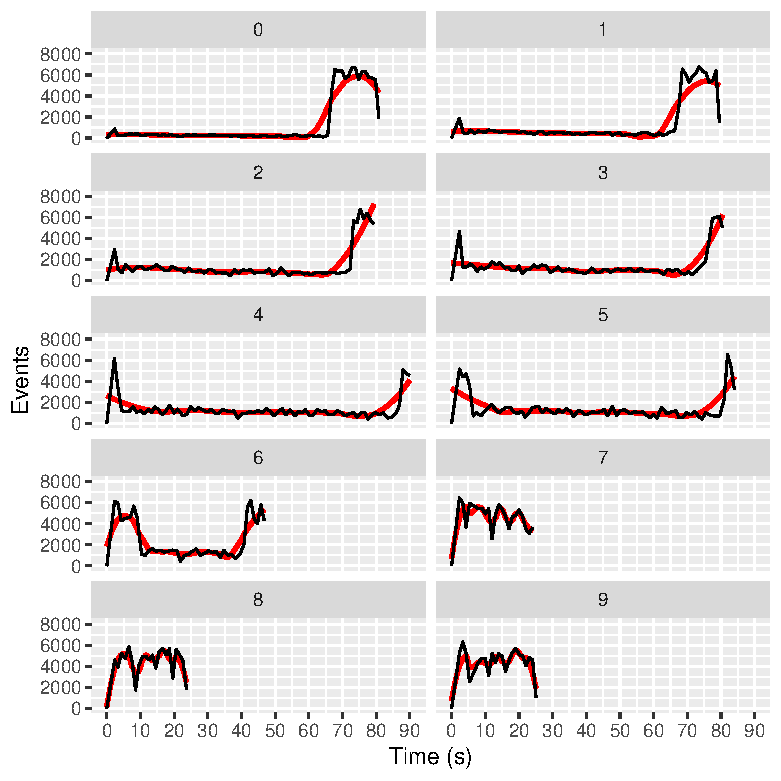
\includegraphics[width=\textwidth]{gfx/config-comparison_100k}
        \caption{}
        \label{fig:evaluation:performance:config-comparison_100k}
\end{figure}


\section{Null Hypothesis}

%short: what is the null hypothesis -- cf. \cite{Kohavi2009}
%\cite{Kohavi2013a}: To validate an experimentation system, we recommend that A/A tests be run regularly to test that the experimental setup and randomization mechanism is working properly. An A/A test, sometimes called a null test (Peterson 2004), exercises the experimentation system, assigning users to one of two groups, but exposes them to exactly the same experience.

% experimental set-up

% execution

% results

\section{Validity}
\label{sec:evaluation:validity}

\cite{Easterbrook2008a}: Construct, internal \& evernal validity, reliability

\section{Experimentation Guidelines for IFAS}

This section describes how different types of experiments can be executed using \ac{IFAS}.\todo{this is a kind of "subjective evaluation" -- maybe not the right place for this?}

\begin{description}
\item[A/B test]
\item[Null hypothesis] aka A/A test \cite{Kohavi2009}
\item[Collecting metrics] i.e. usage data in general, e.g. scroll time
\item[Collecting performance metrics(?)] (unclear, maybe into future work)
\item[Survey(?)] (maybe into future work, POC: Create user interview via \ac{IFAS})
\end{description}

